\section{System Model}
\label{sec:system_model}

\begin{figure}[thbp]
  \centering
  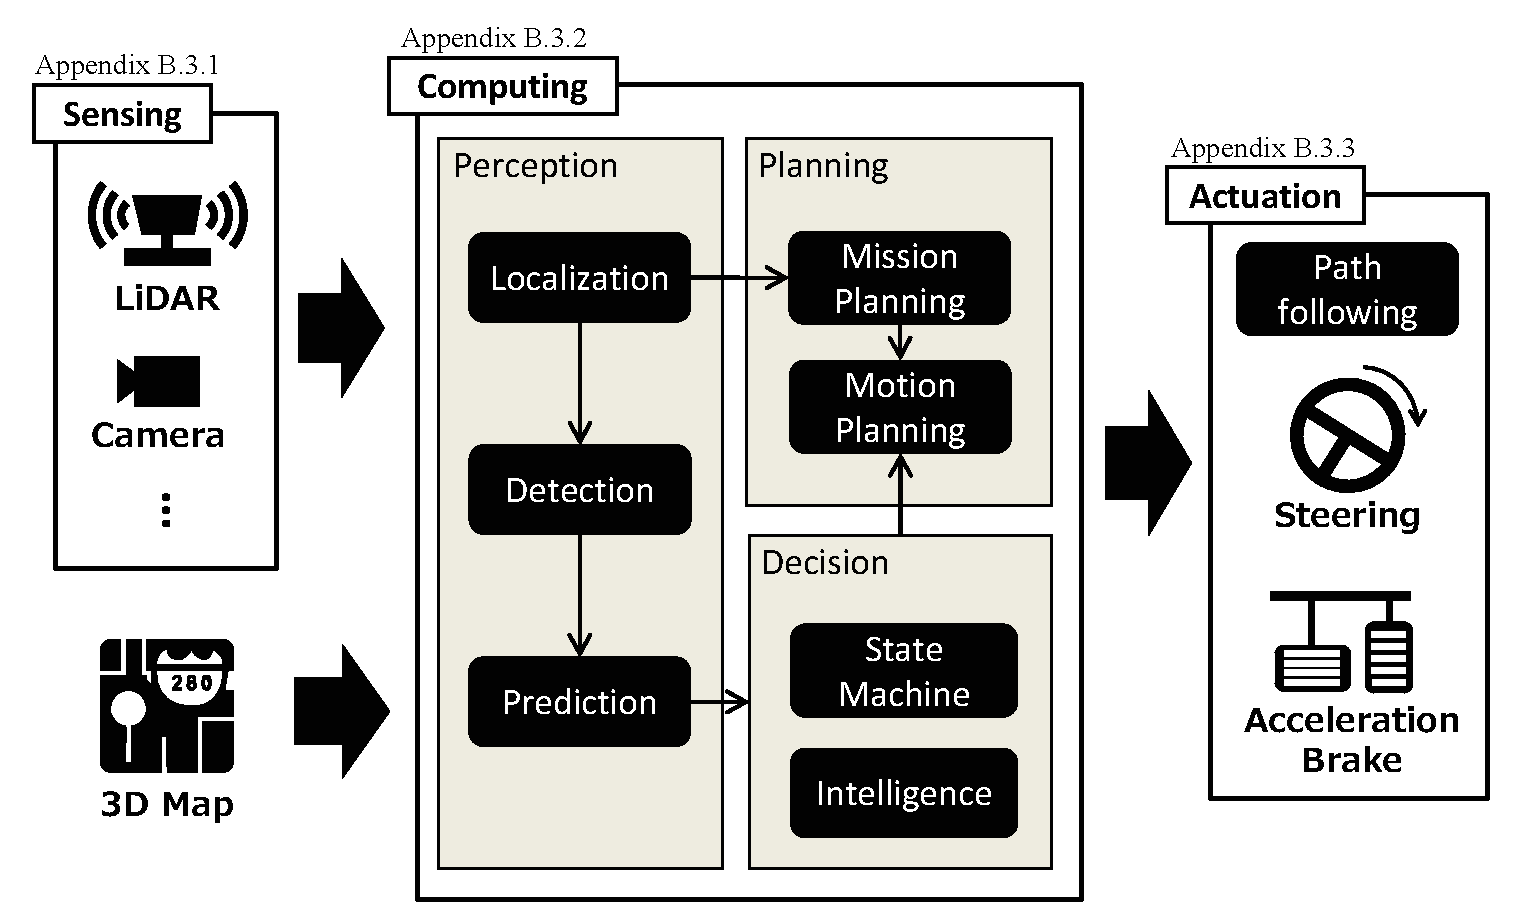
\includegraphics[width=0.9\linewidth]{../figure/Autoware/system_model.eps}
  \caption{\label{fig:system_model}
    Basic control and data flow of autonomous vehicles.}
\end{figure}

Autonomous vehicles as cyber-physical systems can be abstracted into
sensing, computing, and actuation modules, as shown in Figure
\ref{fig:system_model}.
Sensing devices, such as laser scanners (LiDAR) and cameras, are typically used for self-driving in urban areas.
Actuation modules handle steering and stroking whose
twisted control commands that are typically generated by the path following module.
Computation is a major component of self-driving technology.
Scene recognition, for instance, requires the localization, detection, and
prediction modules, whereas path planning is handled by mission-based and
motion-based modules.
Each module employs its own set of algorithms.
The modules implemented in Autoware are discussed in Section
\ref{sec:algorithms}.

Figure \ref{fig:system_model} shows the basic control and data flow for an
autonomous vehicle.
Sensors record environmental information that serves as input data for the
artificial intelligence core.
3D maps are becoming a commonplace for self-driving systems, particularly,
in urban areas as a complement to the planning data available from sensors.
External data sources can improve the accuracy of
localization and detection without increasing the complexity of the vehicle's algorithms.
Artificial intelligence cores typically output values for angular and linear
velocities, which serve as commands for steering and stroking, respectively.

\section{System Stack}

\begin{figure*}[thbp]
  \centering
  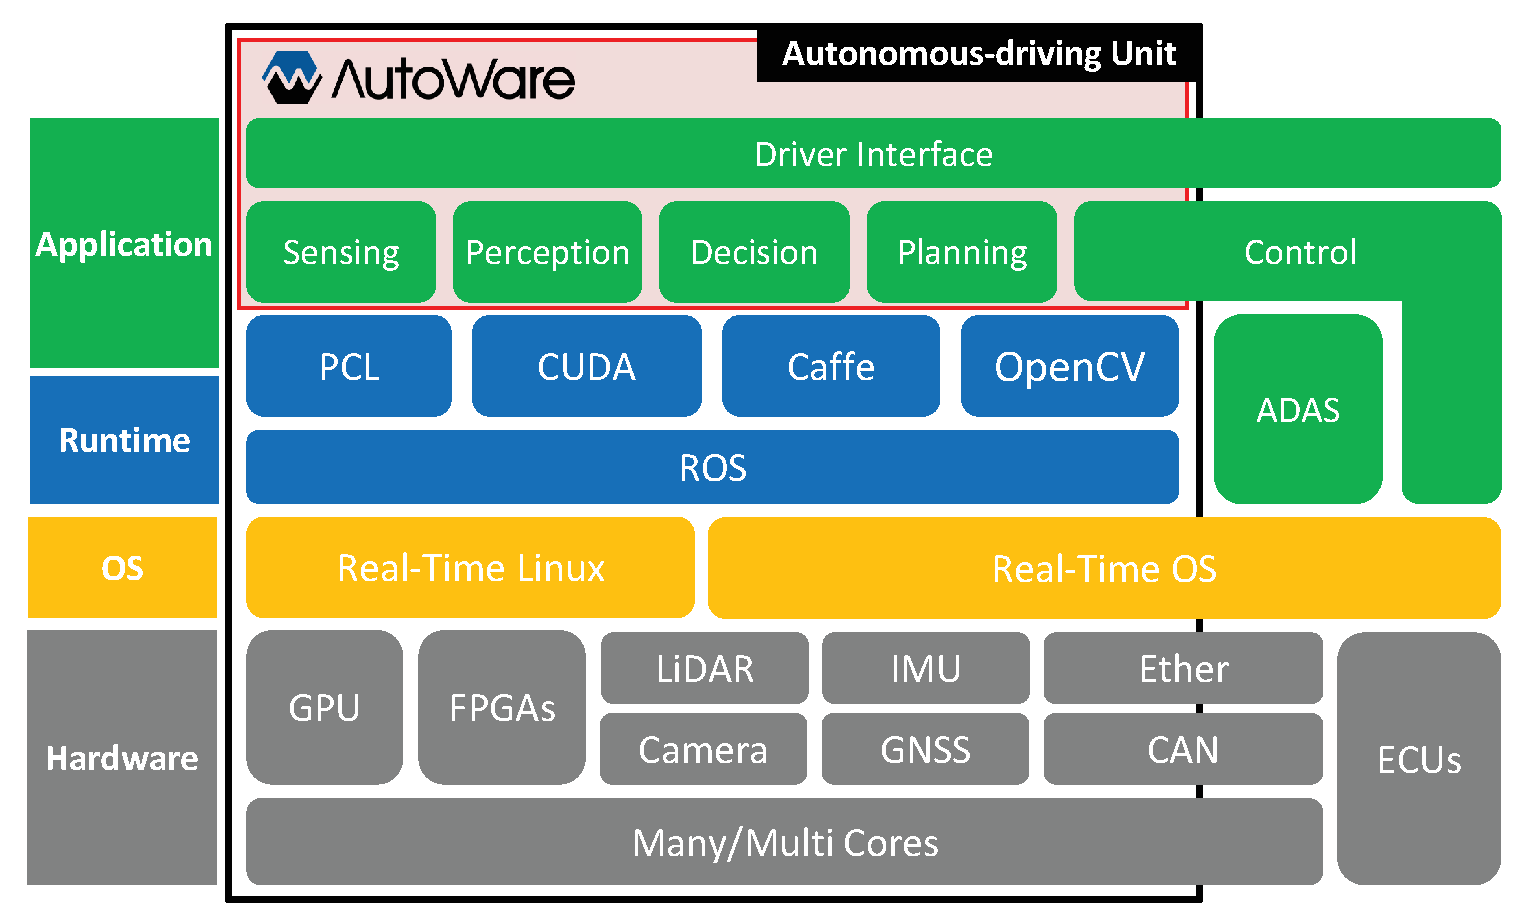
\includegraphics[width=0.9\linewidth]{../figure/Autoware/system_stack.eps}
  \caption{\label{fig:system_stack}
  Complete system stack of autonomous vehicles using Autoware.}
\end{figure*}

Autonomous is designed for a complete software stack for autonomous vehicles that are implemented with open-source software, as shown in
Figure~\ref{fig:system_stack}.
The self-driving technology discussed herein is intended for vehicles that are driven in
urban areas instead in freeways or highways.
I contributed to the development of Autoware, a popular
open-source software project developed for autonomous
vehicles intended for using in urban areas.
Autoware is based on Robot Operating System (ROS) and other
well-established open-source software libraries, as shown in
Figure~\ref{fig:system_stack}.
Appendix A provides a brief overview of ROS.
Point Cloud Library (PCL) \cite{pcl} is mainly used to manage LiDAR
scans and 3D mapping data, in addition to performing data-filtering and visualization functions.
CUDA \cite{cuda} is a programming framework developed by NVIDIA and is used for general-purpose
computing on GPUs (GPGPU).
To handle the computation-intensive tasks involved in self-driving, GPUs running CUDA are
promising solutions for self-driving technology, though this thesis does
not focus on them.
Caffe \cite{jia2014caffe}, \cite{caffe} is a deep learning
framework designed with expression, speed, and modularity in mind.
OpenCV \cite{opencv} is a popular computer vision library for image
processing.

Autoware uses such tools to compile a rich set of software packages, including sensing,
perception, decision making, planning, and control modules.
Many drive-by-wire vehicles can be transformed into autonomous vehicles
with an installation of Autoware.
In several countries, successful implementations of Autoware have been tested for
autonomous vehicles that are driven for long distances in urban
areas.
Recently, automotive manufacturers and suppliers have begun
implementing Autoware as a baseline for prototype autonomous vehicles.

This section briefly introduces the hardware components that are generally installed in autonomous vehicles.
Commercially available vehicles require minor modifications for a successful application of
our software stack.
This will enable us to control the vehicles using external computers through
a secure gateway and install sensors on the vehicles.
The vehicle, computers, and sensors can be connected by Controller Area Network
(CAN) bus, Ethernet, and/or USB 3.0.
However, the specifications of sensors and computers required for a particular application depend closely on
specific functional requirements of the autonomous vehicle.
Autoware supports range sensor, and I chose Velodyne HDL-32e LiDAR scanners and PointGrey
Grasshopper3 cameras for our prototype system.
Autoware also supports a range of processors.
Many users run Autoware on desktops and laptops.
The NVIDIA DRIVE PX2 is used herein though our previous
study ported Autoware to another embedded computing platform,
the Kalray Massively Parallel Processor Array
(MPPA)~\cite{yuya2017exploring}. 

\section{Algorithms}
\label{sec:algorithms}

This section briefly discusses Autoware modules marked in
Figure~\ref{fig:system_model} emphasizing on the modules
that are developed and extended for using in DRIVE PX2.
The remaining models of Autoware can be studied on its
project repository~\cite{autoware}.
Note that Autoware is designed for autonomous vehicles to be used in urban areas, so additional modules
may be required for vehicles driven on freeways or highways.
Discussions of the accuracy and optimization for each algorithm are beyond
the scope of this study.

\subsection{Sensing}
\label{sec:sensing}
Our system recognizes road environments using
LiDAR scanners, cameras, radars, and GPS/IMU data.
LiDAR scanners and cameras are used as primary sensors.
LiDAR scanners measure the distance by illuminating a
target with pulsed lasers and measuring the timing of reflected pulses.
Point-cloud data from LiDAR units can be used to create digital
3D representations of the environment.
Cameras are often used to recognize traffic lights and objects and are sometimes
superior to LiDAR scanners in recognizing object features and providing better sampling rates.

Raw point-cloud data requires filtering and pre-processing.
Autoware applies the Normal Distributions Transform (NDT)
algorithm \cite{biber2003normal} for 3D point-cloud pre-processing. 
The data can be reduced to approximate
points in the lattice by replacing the original points with voxels in a computational lattice \cite{magnusson2009three}.
This filter is applied before localization, detection, and
mapping.

Radars and GPS/IMU data can be used to refine the
localization, detection, and mapping processes.
Radars are already available in commercial vehicles and are often used
for ADAS safety applications.
GPS/IMU data can be coupled with gyroscope sensors and odometers to refine the
positioning information.

\subsection{Computing}
\label{sec:computing}

The computing center is a major component of self-driving
vehicles.
Taking sensor data and 3D maps as inputs, it computes the final
trajectory as the output to actuation modules.
This section explains the computing center in detail from the viewpoints of perception,
decision-making, and planning.

\subsubsection{Perception}
\label{sec:perception}
The perceptual module must estimate the position of the
ego-vehicle in the 3D map and recognize objects in the surrounding scene
including moving objects and traffic signals.

\textbf{Localization}:
The localization submodule has a great effect on the
reliability of the autonomous system, as it senses the vehicle's position within the environment.
Autoware performs localization by scan matching between 3D maps and
LiDAR scanners, which allows precision on the order of a few centimeters for
position and rotation.
Autoware uses the NDT \cite{biber2003normal} algorithm for
localization.
The computational cost of the NDT algorithm is not affected by the map
size, thereby enabling a real-time application of high-definition and high-resolution 3D data.
To be precise, the 3D version of NDT is used for scan matching
over filtered 3D point-cloud data and 3D map data with PCL, as shown
in Figure \ref{fig:rviz_autoware} (b) \cite{magnusson2009three}.
As a result, Autoware can localize the position of ego-vehicles that are located within a few centimeters.

Localization is also a key technique for 3D mapping.
If autonomous vehicles are localized precisely in real-time, 3D maps can
be generated and updated continuously by uploading 3D point-cloud
data acquired from every 3D LiDAR scan.
This approach is often referred to as Simultaneous Localization And
Mapping (SLAM).

Although Autoware also supports another well-known algorithm called iterative closest point,
the NDT algorithm is used for both localization and mapping herein.
Autoware allows users to choose the best algorithm
for their system.

% \begin{figure}[htbp]
%     \centering
%     \includegraphics[width=1.0\linewidth]{../figure/Autoware/rviz_localization.eps}
%     \caption{\label{fig:rviz_localization}
%     NDT scan matching localization using a 3D map and a 3D LiDAR scan.}
% \end{figure}
  
\textbf{Detection}:
Autoware must next detect surrounding objects, such as
vehicles, pedestrians, and traffic signals, to avoid accidents or
violations of traffic rules.
Autoware recognizes traffic signals and lights; however, this section primarily focus on moving objects such as vehicles and pedestrians.
Autoware supports deep learning \cite{liu2016ssd},
\cite{DBLP:journals/corr/RedmonF16} and pattern recognition
\cite{felzenszwalb2010object} for object detection
using libraries such as Caffe and OpenCV.
As shown in Figure \ref{fig:rviz_autoware} (c), Autoware primarily use SSD \cite{liu2016ssd} and the You only look once (Yolo2) algorithms
\cite{DBLP:journals/corr/RedmonF16}, which are based on deep learning.
They are unified frameworks for object detection that use a single neural
network and allow real-time object detection.
Autoware also includes a pattern recognition algorithm based on Deformable
Part Models (DPM) \cite{felzenszwalb2010object}, which searches and scores the
histogram of oriented gradients features of target objects in 2D images \cite{dalal2005histograms}.

In addition to 2D image processing, our prototype also uses point-cloud data scanned from a
3D LiDAR scanner to detect objects using Euclidean clustering.
Point cloud clustering allows Autoware to measure the distance between objects and the vehicle.
This distance information can be used to range and track objects that are
classified by 2D image processing algorithms.

Assuming that localization is precise and a 3D map has been constructed for the area
wherein the autonomous vehicle is driven, I improve upon Autoware's accuracy at recognizing traffic signals and traffic lights.
Autoware determines the exact road area in the image by projecting the 3Dmap onto an image originating at the current position.
The region of interest (ROI) for image
processing can be constrained to this area, thereby reducing execution time and
the occurrence of false positives.
To obtain ROIs, I calibrated the 3D LiDAR data to the 2D camera in advance, as
this calibration cannot be performed by the prototype while operating.
Our ROI approach can recognize traffic signals from 2D images, as shown in Figures \ref{fig:rviz_autoware} (f) and (g).
In general, traffic light recognition is the most
difficult problem associated with autonomous vehicles.
Autoware can accurately recognize traffic lights using 3D mapping data and precise
localization.

% \begin{figure}[htbp]
%     \centering
%     \includegraphics[width=1.0\linewidth]{../figure/Autoware/rviz_detection.eps}
%     \caption{\label{fig:rviz_detection}
%     Object detection and traffic-light recognition with sensor fusion: (a) results of SSD objects detection, (b) projection of the 3D point-cloud data onto the image, (c) traffic-light positions of 3D map, (d) ROI and results of traffic-light recognition.}
% \end{figure}


\textbf{Prediction}:
Because the object-detection algorithm processes each frame of the image and point-cloud data, the results must be associated with other frames in the time series to predict the trajectories of moving objects for mission and motion planning.

Kalman Filter or Particle Filter can be used to solve this inverse problem.
Kalman Filter is used if the assumption that the autonomous vehicle is driving at constant velocity while tracking moving objects holds true \cite{kalman1960new}.
The computational cost of this filter is lightweight, thereby making it suitable for real-time processing.
Particle Filter, in contrast, can be applied to nonlinear tracking scenarios, which are appropriate for realistic driving \cite{arulampalam2002tutorial}.
Our platform uses both Kalman and Particle Filter, depending on the given scenario.
They are used for tracking in both the 2D image plane and the 3D point-cloud domain.

The detected and tracked objects in the 2D image can be combined with clustered and tracked objects obtained from the 3D LiDAR sensor;
this process is referred to as sensor fusion with projection and re-projection.
The sensor fusion parameters are determined in the lab while calibrating the LiDAR scanner to the 2D camera.

Autoware support scene recognition with sensor fusion of the camera and 3D LiDAR sensor.
You can then project the 3D point-cloud information obtained by the 3D LiDAR sensor onto 2D images, thereby adding depth information to the image and filtering for ROIs.
Figures \ref{fig:rviz_autoware} (d) and (e) show the results of projection and adding bounding boxes to clustered 3D point-cloud objects projected onto the image.

The detected and tracked objects on the image can be re-projected onto the 3D point-cloud coordinates using the same extrinsic parameters.
You also use the reprojected object positions to determine the motion plan and, partially, the overall trajectory.

\subsubsection{Decision}
\label{sec:decision}

After Autoware recognizes relevant obstacles and traffic signals in the environment, it can plot the trajectories of other moving objects and make decisions about mission and motion planning.
The prediction and comprehensive decision-making modules are under development in our self-driving platform.

Autoware adopt a state machine and machine learning intelligence for understanding, forecasting, and decision-making in response to road scenarios.
Our platform enables drivers to supervise the state of the vehicle while making comprehensive decisions for the planning modules to execute.

\subsubsection{Planning}
This module plans trajectories following the decision-making module's output.
Autoware break path planning into mission and motion planning.
The platform plans a global trajectory based on the current location and specified destination and conducts basic local motion planning to determine the overall trajectory.
Available graph-search algorithms include hybrid-state A* \cite{dolgov2010path}, and trajectory generation algorithms include \cite{nagy2001trajectory} such as lattice-based algorithms \cite{darweesh2017open}.
% A demonstration video of the adaptation of OpenPlanner to Autoware can be seen at: https://www.youtube.com/watch?v=FKM8v79X3_s
A motion planner suited to the decision-making module must be chosen, depending on the road scenario.

\textbf{Mission planning}:
Drawing upon traffic laws, the our mission planner uses a rule-based mechanism to autonomously assign a path trajectory for purposes such as lane changes, merges, and passing.
This mechanism is not completely autonomous in our platform.
The high-definition 3D map contains static road information used for navigation and global planning.
In more complex scenarios, such as parking and recovering from operational mistakes, the driver can supervise the path.
In either case, once the path is assigned, the local motion planning module is launched.

The basic goal of the mission planner is to drive in a cruising lane over the route provided by a commercially available navigation application based on the high-definition 3D map.
The vehicle changes lanes only when it passes a preceding vehicle or approaches an intersection followed by a turn.

\textbf{Motion planning}:
The motion planner adjusts self-driving in response to driving behavior, which is not common across users and environments.
Hence, the prototype platform currently provides only a basic motion-planning strategy to allow us to build a high-level intelligence for making comprehensive decisions.
Constrained by the current and goal states of the vehicle, a feasible trajectory must be generated dynamically from the travelable area based on the 3D map and with consideration of surrounding objects and traffic rules.

In unstructured environments, such as parking lots, Autoware can use graph-search algorithms, such as A* \cite{hart1968formal} and hybrid-state A* \cite{dolgov2010path}, to find the minimum-cost path to the goal using a cost map, as shown in Figures \ref{fig:rviz_autoware} (h) and (i).
Although graph-search algorithms consume a great deal of processing power, they can analyze complex scenarios.
In contrast, in structured environments, such as roads and traffic lanes, vertices are likely to be dense and and irregularly distributed, which constrains the options for feasible headings.
Therefore,for urban areas, the prototype uses spatiotemporal lattice-based algorithms to adapt motion plans to the environment \cite{mcnaughton2011motion}.
State-of-the-art research encourages the implementation of these algorithms \cite{urmson2008autonomous}.
Trajectories for obstacle avoidance and lane changes must be calculated in real time using fast algorithms \cite{pivtoraiko2009differentially}, \cite{mcnaughton2011motion}, and they can be selected with an evaluation function, as shown in Figure \ref{fig:rviz_autoware} (j).

\subsection{Actuation}
\label{sec:actuation}
Our autonomous vehicle prototype follows the path generated by the motion planner.

\textbf{Path following}:
The pure pursuit algorithm \cite{coulter1992implementation} acutuates our prototype.
The pure pursuit algorithm breaks down the path into multiple waypoints.
During every control cycle, the module searches for the closest waypoint in the direction of travel.
The search extends beyond the specified threshold distance to reduce the change in angle that is required when returning onto the path from a deviation.
As shown in Figure \ref{fig:rviz_autoware} (k), the velocity and angle of the next movement are set to values that bring the vehicle to the selected waypoint following a predefined curvature.

The target waypoint is updated accordingly until the goal is reached.
The vehicle follows these updated waypoints until it reaches the user-specified goal.
If the control of acceleration steps is not aligned with the velocity and angle output of the pure pursuit algorithm because of noise, the vehicle can temporarily deviate from the planned trajectory.
Although the current iteration of our prototype uses a simple PID controller to actuate the vehicle, parameters highly depend on the vehicle and the controller is not sufficient to control the vehicle smoothly.
Localization errors can also cause gaps between the vehicle state and the outputs of the pure pursuit algorithm.
As a result, the vehicle could collide with unexpected obstacles.
To cope with this scenario, the path following module ensures a minimum distance between the vehicle and detected obstacles, overriding the planned trajectory.
Our motion planner also updates the waypoints accordingly, considering obstacles in the upcoming travel lane.

\clearpage

\begin{figure*}[thbp]
  \centering
  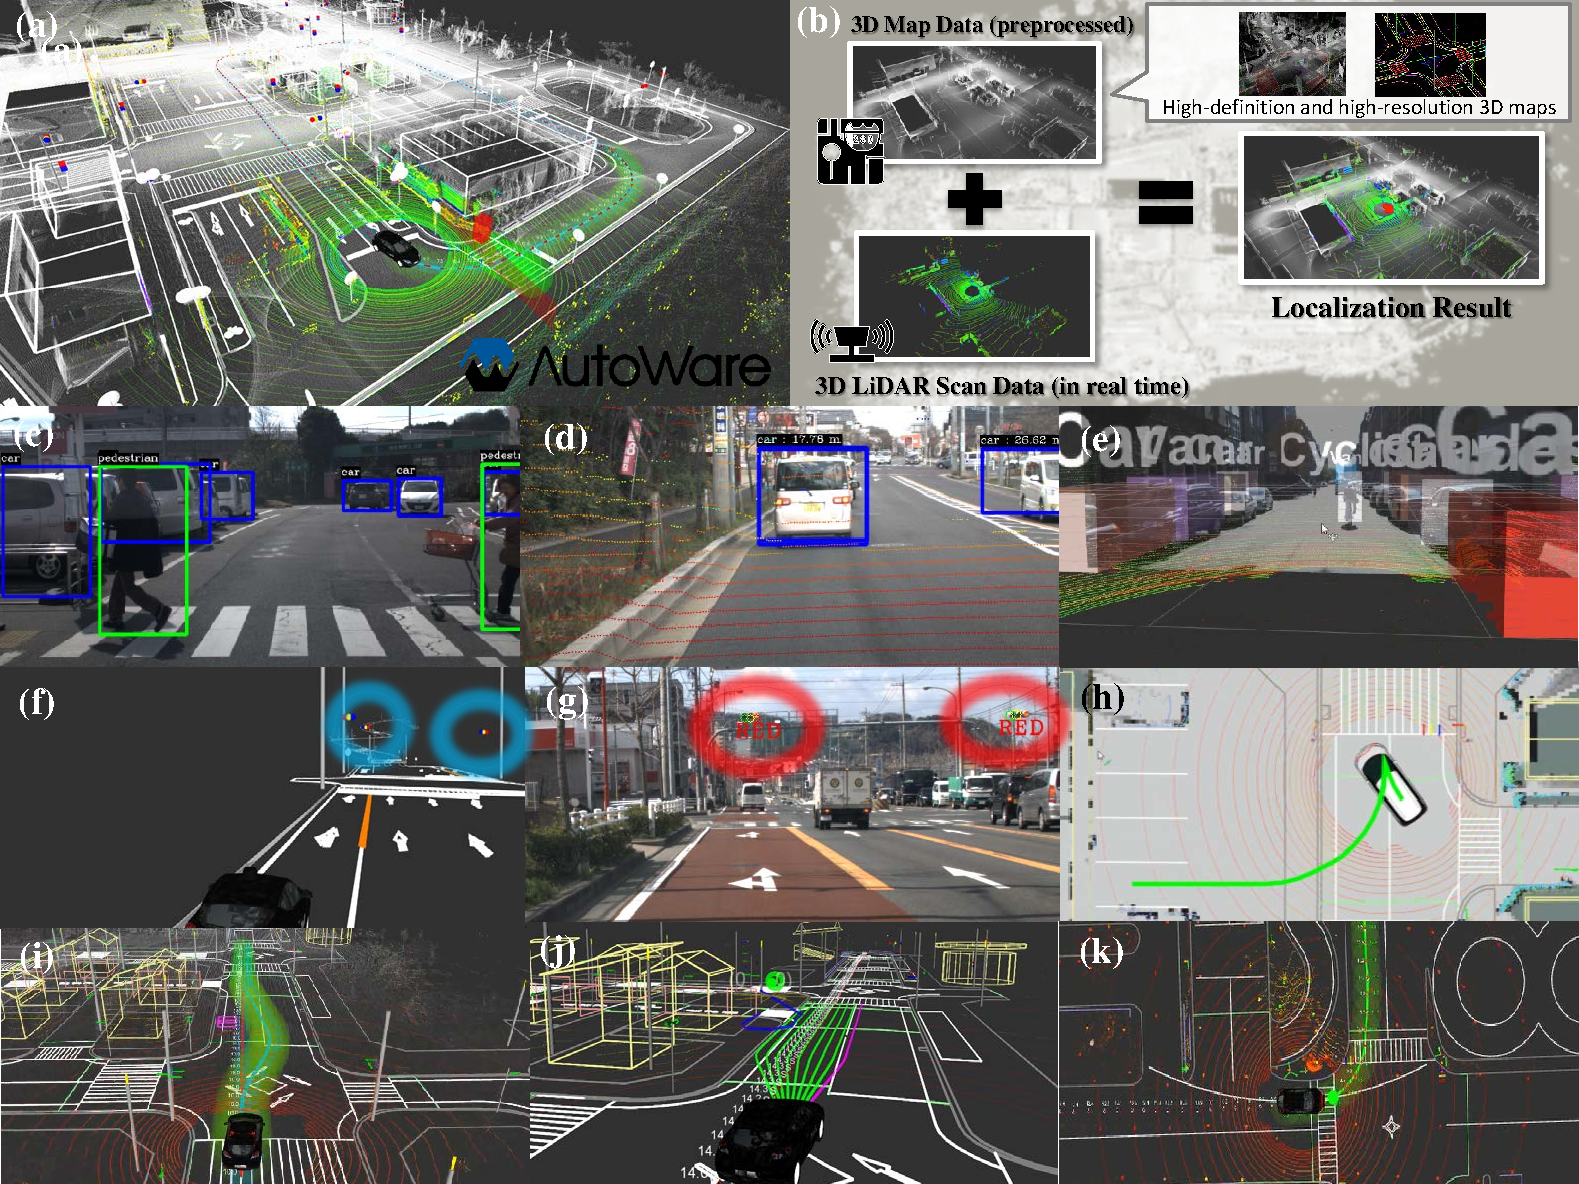
\includegraphics[width=1.0\linewidth]{../figure/Autoware/rviz_autoware.eps}
  \caption{\label{fig:rviz_autoware}
  Self-driving software packages in Autoware:
  (a) RViz visualization with high-definition and high-resolution geographical information,
  (b) NDT scan matching localization using a 3D map and a 3D LiDAR scan,
  (c) deep learning based object detection with the You only look once (Yolo2) algorithms,
  (d) projection of the 3D point-cloud data onto the image,
  (e) calibrated data fusion for LiDAR clouds and images data,
  (f) traffic light positions extracted from the 3D map,
  (g) traffic light recognition with the region of interest marked,
  (h) trajectory planning in a parking lot using hybrid-state A* search,
  (i) trajectory planning for object avoidance using hybrid-state A* search,
  (j) trajectory generation for object avoidance using the lattice-based algorithm, and
  (k) steering angular velocity calculations for path following using the pure pursuit algorithm.}
\end{figure*}
